% Standalone source: all explanatory figures are TikZ vector graphics.
% Compile: pdflatex zeta-pratt-spherical-shells-en.tex (twice).
\documentclass[11pt,a4paper]{article}
\usepackage[T1]{fontenc}
\usepackage[utf8]{inputenc}
\IfFileExists{english.ldf}{\usepackage[english]{babel}}{%
  \usepackage{babel}\babelprovide[main,import=en]{english}}
\usepackage{lmodern,microtype,amsmath,amssymb,mathtools}
\usepackage[a4paper,left=22mm,right=22mm,top=22mm,bottom=22mm]{geometry}
\usepackage{tikz}
\usetikzlibrary{arrows.meta,calc,positioning,decorations.pathreplacing}
\usepackage{booktabs,array,tabularx,caption,fancyhdr,titlesec}
\usepackage[most]{tcolorbox}
\usepackage{hyperref}
\definecolor{navy}{HTML}{142A43}
\definecolor{teal}{HTML}{087F8C}
\definecolor{amber}{HTML}{BD721B}
\definecolor{violet}{HTML}{7656A1}
\definecolor{muted}{HTML}{566775}
\definecolor{pale}{HTML}{F1F7F8}
\hypersetup{colorlinks=true,linkcolor=teal,urlcolor=teal,
  pdftitle={A Zeta-Pratt Fractal as a Volume of Spherical Shells},
  pdfsubject={Zoom, stereographic projection, camera and attenuation}}
\setlength{\parindent}{0pt}
\setlength{\parskip}{5.5pt}
\setlength{\headheight}{15pt}
\setlength{\emergencystretch}{1.5em}
\renewcommand{\arraystretch}{1.18}
\titleformat{\section}{\Large\sffamily\bfseries\color{navy}}{\thesection}{.7em}{}
\titlespacing*{\section}{0pt}{8pt}{10pt}
\titleformat{\subsection}{\normalsize\sffamily\bfseries\color{navy}}{}{0pt}{}
\titlespacing*{\subsection}{0pt}{9pt}{3pt}
\pagestyle{fancy}
\fancyhf{}
\fancyhead[L]{\small\sffamily\color{muted}Zeta-Pratt \enspace / \enspace Spherical-Shell Model}
\fancyhead[R]{\small\sffamily\color{muted}Mathematical Description}
\fancyfoot[L]{\small\sffamily\color{muted}Symbolic figures, not a fractal simulation}
\fancyfoot[R]{\small\sffamily\color{muted}\thepage}
\renewcommand{\headrulewidth}{.3pt}
\captionsetup{font=small,labelfont={bf,sf},textfont={color=muted},skip=5pt,hypcap=false}
\numberwithin{equation}{section}
\newcommand{\R}{\mathbb R}
\newcommand{\C}{\mathbb C}
\newcommand{\Sph}{\mathbb S^2}
\newcommand{\vct}[1]{\boldsymbol{#1}}
\newcommand{\F}{\mathcal F}
\newcommand{\dd}{\mathop{}\!\mathrm d}
\newcommand{\SO}{\mathrm{SO}(3)}
\newtcolorbox{modelbox}[1][]{colback=pale,colframe=teal!45,
  boxrule=.5pt,arc=2mm,left=9pt,right=9pt,top=7pt,bottom=7pt,#1}
\tikzset{>=Latex,ray/.style={->,line width=1pt,teal},
  symbol/.style={font=\small\sffamily,text=navy},
  note/.style={font=\footnotesize\sffamily,text=muted,align=center},
  pics/flower/.style={code={
    \draw[teal!85,line width=.7pt,fill=teal!8]
      plot[domain=0:360,samples=101,smooth,variable=\t]
        ({(.29+.14*cos(5*\t))*cos(\t)},
         {(.29+.14*cos(5*\t))*sin(\t)});
    \foreach \a in {0,72,144,216,288}
      \draw[violet!70,line width=.45pt] (0,0) -- (\a:.4);
    \fill[amber] (0,0) circle (.045);
  }}}

\begin{document}
\thispagestyle{fancy}
{\fontsize{27}{31}\selectfont\sffamily\bfseries\color{navy}
  A Zeta-Pratt Fractal\par as a Three-Dimensional Volume\par}
\vspace{5pt}
{\large\sffamily\color{teal}Each infinitesimal spherical shell is a different zoom level.\par}
\vspace{5pt}
{\small\color{muted}Elaboration of the proposed model \enspace | \enspace 5 October 2026}

\section{The Spatial Field}
The observer is located at the fixed center $\vct o\in\R^3$.
The image fills space: the same planar Zeta-Pratt pattern lies on every spherical
shell, but with a zoom that depends on the radius. Greater depth can correspond
simultaneously to greater magnification and lower brightness.

\begin{center}
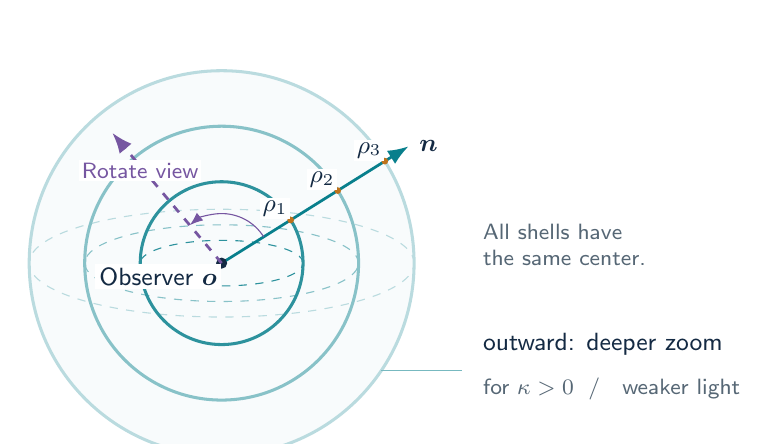
\begin{tikzpicture}[scale=.94]
  \fill[teal!3] (0,0) circle (2.6);
  \foreach \r/\col in {2.6/teal!28,1.85/teal!48,1.1/teal!85}{
    \draw[\col,line width=1.1pt] (0,0) circle (\r);
    \draw[\col,dashed] (0,0) ellipse ({\r} and {\r*.28});
  }
  \draw[ray] (0,0) -- (32:2.98) node[symbol,right] {$\vct n$};
  \foreach \r/\lab in {1.1/1,1.85/2,2.6/3}{
    \fill[amber] (32:\r) circle (.045);
    \node[symbol,above left,fill=white,inner sep=1pt] at (32:\r) {$\rho_{\lab}$};
  }
  \fill[navy] (0,0) circle (.075);
  \node[symbol,below left,fill=white,inner sep=1.5pt] at (0,0) {Observer $\vct o$};
  \draw[ray,violet,dashed] (0,0) -- (130:2.3);
  \draw[->,violet] (32:.67) arc (32:130:.67);
  \node[note,text=violet,fill=white,inner sep=1pt] at (-1.1,1.25) {Rotate view};
  \draw[teal!55] (2.15,-1.45) -- (3.25,-1.45);
  \node[symbol,anchor=west] at (3.4,-1.1) {outward: deeper zoom};
  \node[note,anchor=west,align=left] at (3.4,-1.7) {for $\kappa>0$\; / \; weaker light};
  \node[note,anchor=west,align=left] at (3.4,.25) {All shells have\\the same center.};
\end{tikzpicture}
\captionof{figure}{Symbolic cross-section through the volume. The drawn shells
represent a continuous spectrum of radii.}
\end{center}

For $\vct x\ne\vct o$, set
\[
\rho=\|\vct x-\vct o\|,\qquad
\vct n=\frac{\vct x-\vct o}{\rho}\in\Sph.
\]
\begin{modelbox}
\textbf{Basic formula: direction becomes a complex coordinate, depth becomes zoom.}
\begin{equation}\label{eq:field}
 C_{\vct o}(\vct x)=a(\rho)\,
 \F\!\left(z_\ast+\frac{\sigma(\vct n)}{Z(\rho)}\right).
\end{equation}
\end{modelbox}
\begin{tabularx}{\linewidth}{@{}>{$}l<{$}X@{}}
 \F(z) & RGB color of the planar Zeta-Pratt pattern, componentwise in $[0,1]$.\\
 z_\ast\in\C & Fixed target point about which the pattern is magnified.\\
 \sigma(\vct n) & Stereographic coordinate of the direction; see Section 3.\\
 Z(\rho)>0,\ a(\rho)\ge0 & Zoom factor and brightness factor of the shell.\\
\end{tabularx}

\newpage
\section{The Zeta-Pratt Texture}
\subsection{The Given Family}
For positive integer indices, the recursive definitions are
\begin{equation}
 f_1(z)=1,\qquad f_2(z)=z,\qquad
 f_p(z)=1+f_{p-1}(z)\quad(p>2\text{ prime}),
\end{equation}
and for composite $n$, the prime factorization
\begin{equation}
 f_n(z)=\prod_{p\mid n}f_p(z)^{v_p(n)}.
\end{equation}
Here $v_p(n)$ denotes the exponent of $p$ in $n$.
The requested extensions are $f_0(z)=0$ and $f_{-n}(z)=-f_n(z)$.
For a real index $r$ and a complex index $s=a+ib$, set
\begin{align}
 f_r(z)&=(1-t)f_m(z)+t f_{m+1}(z),
 & m&=\lfloor r\rfloor,\quad t=r-m,\\
 f_s(z)&=f_a(z)+i f_b(z).
\end{align}
For fixed $s$, this yields a polynomial in $z$; moreover, $f_s(2)=s$.
The index $r$ must be distinguished here from the spatial depth $\rho$.

\subsection{The Iterated Map of the Existing Image}
We use the composition $\zeta\circ f_s$. In particular, from
$f_4(z)=z^2$, $f_5(z)=z^2+1$, and $f_{1/2}(z)=1/2$:
\begin{modelbox}
\begin{equation}\label{eq:H}
 H(z)=\zeta\!\left(f_{4.5+0.5i}(z)\right)
     =\zeta\!\left(z^2+\tfrac12+\tfrac i2\right),
 \qquad z_{j+1}=H(z_j).
\end{equation}
\end{modelbox}
The zeta function is understood via its meromorphic continuation. Its Dirichlet series
is valid for $\Re w>1$; at $w=1$ it has a simple pole [1].
Thus $H$ has poles at $z^2=(1-i)/2$.

\begin{center}
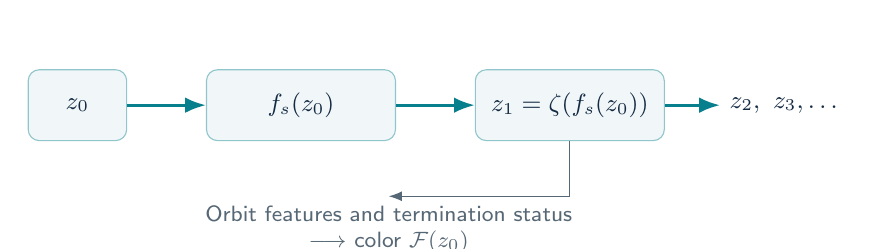
\begin{tikzpicture}[node distance=1cm]
  \node[draw=teal!45,fill=pale,rounded corners,minimum width=1.25cm,minimum height=.9cm,symbol] (a) {$z_0$};
  \node[draw=teal!45,fill=pale,rounded corners,minimum width=2.4cm,minimum height=.9cm,symbol,right=of a] (b) {$f_s(z_0)$};
  \node[draw=teal!45,fill=pale,rounded corners,minimum width=2.4cm,minimum height=.9cm,symbol,right=of b] (c) {$z_1=\zeta(f_s(z_0))$};
  \node[symbol,right=.7cm of c] (d) {$z_2,\ z_3,\ldots$};
  \draw[ray] (a)--(b); \draw[ray] (b)--(c); \draw[ray] (c)--(d);
  \draw[->,muted] (c.south) -- ++(0,-.7) -- ++(-2.3,0)
    node[below,note,align=center] {Orbit features and termination status\\$\longrightarrow$ color $\F(z_0)$};
\end{tikzpicture}
\captionof{figure}{An initial coordinate is iterated and then colored.
The image function $\F$ contains the chosen numerical representation.}
\end{center}

\subsection{What the Color Means}
In practice, evaluation stops after at most $N$ steps:
\[
 \F(z_0)=\operatorname{Palette}
   (\text{status},\text{step count},\text{return test},\arg z_j,\log(1+|z_j|)).
\]
The existing image uses such finite orbit features and numerical termination
thresholds. It is therefore an \emph{orbit representation}; the colors alone
prove neither convergence nor membership in a mathematically exact Julia set.
For the shell model, a fixed, bounded, and measurable image function $\F$ is sufficient.

\newpage
\section{From the Complex Plane to Every Spherical Shell}
The Riemann sphere is the complex plane together with the added point
$\infty$. It provides a natural directional coordinate.
For $\vct n=(n_x,n_y,n_z)\in\Sph$, we use
\begin{equation}\label{eq:stereo}
 \sigma(\vct n)=\frac{n_x+i n_y}{1-n_z},\qquad
 \vct n\ne\vct N:=(0,0,1).
\end{equation}
The south pole $(0,0,-1)$ corresponds to $z=0$, and the north pole $\vct N$ to
$\infty$. This sign convention matches the sphere mapping used so far.

\begin{center}
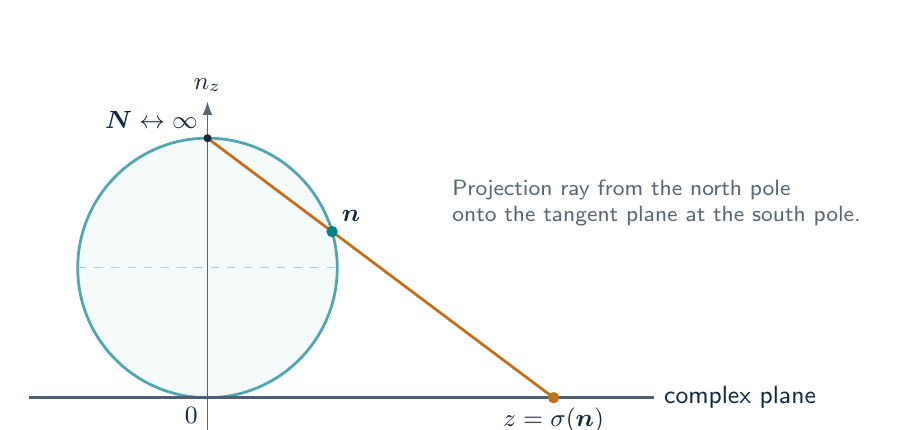
\begin{tikzpicture}[scale=1.03]
  \fill[teal!4] (0,0) circle (1.6);
  \draw[teal!70,line width=1pt] (0,0) circle (1.6);
  \draw[teal!35,dashed] (-1.6,0)--(1.6,0);
  \draw[->,muted] (0,-2.15)--(0,2.05) node[symbol,above] {$n_z$};
  \draw[navy!75,line width=1pt] (-2.2,-1.6)--(5.5,-1.6)
    node[symbol,right] {complex plane};
  \coordinate (N) at (0,1.6);
  \coordinate (P) at (1.536,.448);
  \coordinate (Z) at (4.267,-1.6);
  \draw[amber,line width=1pt] (N)--(Z);
  \fill[navy] (N) circle (.05);
  \node[symbol,above left] at (N) {$\vct N\leftrightarrow\infty$};
  \fill[teal] (P) circle (.07);
  \node[symbol,above right] at (P) {$\vct n$};
  \fill[amber] (Z) circle (.07);
  \node[symbol,below] at (Z) {$z=\sigma(\vct n)$};
  \node[symbol,below left] at (0,-1.6) {$0$};
  \node[note,align=left,anchor=west] at (2.9,.8)
    {Projection ray from the north pole\\onto the tangent plane at the south pole.};
\end{tikzpicture}
\captionof{figure}{Stereographic projection in a two-dimensional cross-section.
For the formula, the plane is coordinatized at half the geometric scale.}
\end{center}

The inverse map for $z=u+iv$ is
\begin{equation}
 \sigma^{-1}(z)=\frac{(2u,\,2v,\,u^2+v^2-1)}{1+u^2+v^2}.
\end{equation}
Direct substitution gives $\|\sigma^{-1}(z)\|=1$ and
$\sigma(\sigma^{-1}(z))=z$. On a shell of radius $\rho$,
this directional vector becomes $\vct x=\vct o+\rho\vct n$.

\subsection{The Texture of a Single Shell}
We write
\begin{equation}\label{eq:shell}
 T_\rho(\vct n)=\F\bigl(A_\rho(\sigma(\vct n))\bigr),\qquad
 A_\rho(z)=z_\ast+\frac{z}{Z(\rho)}.
\end{equation}
$A_\rho$ is an affine Möbius transformation of the Riemann sphere [2].
It shifts the target of the excerpt and reduces the sampled distances in the plane.
The actual spherical shell is a copy of the direction sphere; the spatial radius
controls the zoom through $Z(\rho)$.

\subsection{Projection Pole and Center}
The coordinate chart has a pole at the north pole. A second chart
$w=1/z=(n_x-i n_y)/(1+n_z)$ covers its neighborhood, but provides
\emph{no} automatic continuous extension of the fractal color to $z=\infty$.
For an image defined everywhere, a fixed color can be assigned to the single
projection pole. Likewise, one may set $C_{\vct o}(\vct o)=0$; the direction
is undefined there. Both are rendering rules.

\newpage
\section{Depth as a Logarithmic Zoom Coordinate}
A simple model choice is
\begin{modelbox}
\begin{equation}\label{eq:zoom}
 Z(\rho)=Z_0e^{\kappa\rho},\qquad Z_0>0,\quad\kappa\in\R.
\end{equation}
\end{modelbox}
Then
\begin{equation}
 \log Z(\rho)=\log Z_0+\kappa\rho,\qquad
 \frac{Z(\rho+\Delta\rho)}{Z(\rho)}=e^{\kappa\Delta\rho}.
\end{equation}
Shells of equal thickness therefore correspond to equal \emph{multiplicative}
zoom steps. For $\kappa>0$, moving outward zooms in; for $\kappa<0$, it zooms out.
For $\kappa=0$, all shells carry the same texture.

\begin{center}
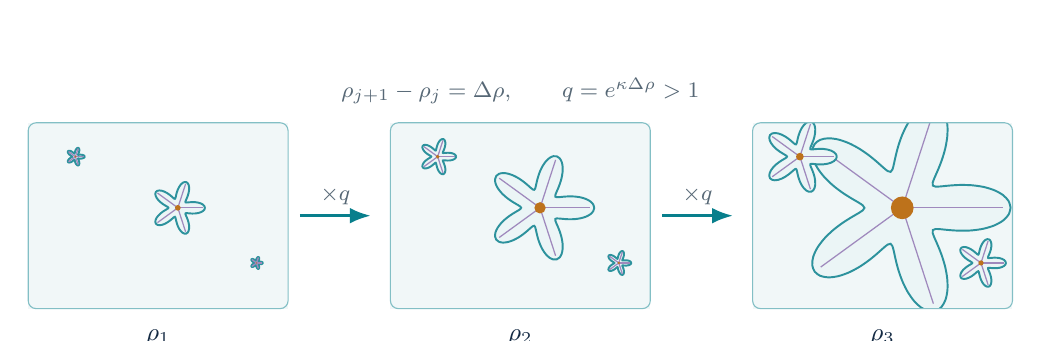
\begin{tikzpicture}
  \foreach \x/\sc/\lab in {0/.8/\rho_1,4.6/1.6/\rho_2,9.2/3.2/\rho_3}{
    \begin{scope}[shift={(\x,0)}]
      \fill[pale] (-1.65,-1.18) rectangle (1.65,1.18);
      \begin{scope}
        \clip (-1.65,-1.18) rectangle (1.65,1.18);
        \pic[scale=\sc] at (.25,.1) {flower};
        \pic[scale=\sc*.34] at (-1.05,.75) {flower};
        \pic[scale=\sc*.23] at (1.25,-.6) {flower};
      \end{scope}
      \draw[teal!50,rounded corners=1mm] (-1.65,-1.18) rectangle (1.65,1.18);
      \node[symbol] at (0,-1.55) {$\lab$};
    \end{scope}
  }
  \draw[ray] (1.8,0)--(2.7,0) node[note,midway,above] {$\times q$};
  \draw[ray] (6.4,0)--(7.3,0) node[note,midway,above] {$\times q$};
  \node[note] at (4.6,1.58) {$\rho_{j+1}-\rho_j=\Delta\rho,\qquad q=e^{\kappa\Delta\rho}>1$};
\end{tikzpicture}
\captionof{figure}{Symbolic magnification sequence. The flower symbols illustrate only
the zoom idea; they are not computed Zeta-Pratt excerpts.}
\end{center}

\subsection{What Happens Along a Ray}
For a fixed direction $\vct n$, the initial coordinate of the fractal iteration is
\begin{equation}\label{eq:zray}
 z(\rho,\vct n)=z_\ast+Z_0^{-1}e^{-\kappa\rho}\sigma(\vct n),\qquad
 \frac{\partial z}{\partial\rho}=-\kappa(z-z_\ast).
\end{equation}
For $\kappa>0$, it approaches the target point $z_\ast$ exponentially as depth
increases. Colors and orbit features can change strongly in the process.
The zoom construction itself does not guarantee exact self-similarity of the pattern.

\subsection{Zoom over a Given Time}
Let $\tau$ be the interaction time and $\nu$ the desired logarithmic zoom rate.
If the camera preferentially displays the depth $\rho_c(\tau)$, set, for $\kappa\ne0$,
\begin{equation}
 \rho_c(\tau)=\rho_c(0)+\frac{\nu}{\kappa}\tau,
 \qquad Z(\rho_c(\tau))=Z(\rho_c(0))e^{\nu\tau}.
\end{equation}
The center $\vct o$ remains fixed. A different depth of the same volume is selected.
For a finite radial range, this motion ends at its boundary; a depth selection is
described in Section 6.

\newpage
\section{The Camera at the Fixed Sphere Center}
A rotation is described by a matrix $Q(\tau)\in\SO$:
\[
 Q^{\mathsf T}Q=\mathrm{Id},\qquad\det Q=1.
\]
For image coordinates $(u,v)$ and a positive camera factor $M(\tau)$, define
\begin{equation}\label{eq:camera}
 \vct n_{\rm cam}(u,v;M)=
 \frac{(u/M,\,v/M,\,1)}{\sqrt{1+(u^2+v^2)/M^2}},\qquad
 \vct n=Q(\tau)\vct n_{\rm cam}.
\end{equation}
Larger $M$ reduces the field angle for an unchanged image area.
The corresponding ray always passes through the same point:
\begin{equation}
 \vct x(\rho;u,v,\tau)=\vct o+\rho\,Q(\tau)\vct n_{\rm cam}(u,v;M(\tau)).
\end{equation}
For an initial view toward the south pole, for example,
$Q(0)=\operatorname{diag}(1,-1,-1)$ is suitable.

\begin{center}
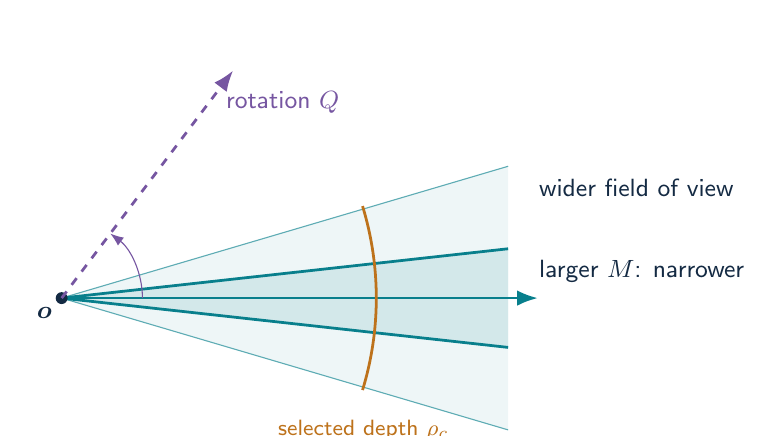
\begin{tikzpicture}[scale=1.08]
  \fill[teal!7] (0,0)--(5.25,-1.55)--(5.25,1.55)--cycle;
  \fill[teal!18] (0,0)--(5.25,-.58)--(5.25,.58)--cycle;
  \draw[teal!65] (0,0)--(5.25,1.55) (0,0)--(5.25,-1.55);
  \draw[teal,line width=1pt] (0,0)--(5.25,.58) (0,0)--(5.25,-.58);
  \draw[ray] (0,0)--(5.6,0);
  \fill[navy] (0,0) circle (.07);
  \node[symbol,below left] at (0,0) {$\vct o$};
  \node[symbol,anchor=west] at (5.5,1.3) {wider field of view};
  \node[symbol,anchor=west] at (5.5,.32) {larger $M$: narrower};
  \draw[ray,violet,dashed] (0,0)--(53:3.35);
  \draw[->,violet] (0:.95) arc (0:53:.95);
  \node[symbol,text=violet] at (2.6,2.3) {rotation $Q$};
  \draw[amber,line width=1pt] (-17:3.7) arc (-17:17:3.7);
  \node[note,text=amber] at (3.55,-1.55) {selected depth $\rho_c$};
\end{tikzpicture}
\captionof{figure}{View rotation and angular zoom change the ray directions.
Depth selection changes which shells are preferentially visible.}
\end{center}

\begin{tabularx}{\linewidth}{@{}l>{\raggedright\arraybackslash}X>{\raggedright\arraybackslash}X@{}}
\toprule
\textbf{Control} & \textbf{Effect} & \textbf{Parameter}\\
\midrule
Rotate & Different viewing direction, same center. & $Q(\tau)$\\
Angular zoom & Narrower section of the spherical panorama. & $M(\tau)$\\
Depth zoom & A different zoom level of the fractal is emphasized. & $\rho_c(\tau)$\\
\bottomrule
\end{tabularx}

\subsection{The Volume Remains Fixed}
As long as $z_\ast$, $Z(\rho)$, $a(\rho)$, and $\F$ remain unchanged, the same field
is being viewed. Only the camera and its depth weighting change. The rotation is
therefore \emph{not} a motion of the sphere center.

The angular zoom $M$ and the fractal zoom $Z$ are different quantities. They may be
coupled, but need not be. By contrast, changing the target point $z_\ast$ or rotating
the texture in formula~\eqref{eq:field} changes the constructed field. For the desired
look inward, a fixed texture with a movable camera and movable depth selection is
sufficient at first.

\newpage
\section{Attenuated Light and Transparent Shells}
For the desired attenuation, choose a positive length scale $\ell$ and
\begin{equation}\label{eq:attenuation}
 a(\rho)=e^{-\rho/\ell}.
\end{equation}
At $\rho=\ell$, the remaining fraction is $e^{-1}\approx0.368$.
This is a prescribed image weighting. The additional relation $\Delta t=\rho/c$
may interpret depth as light-travel time in a static model; it does not follow from
the fractal zoom.

\begin{center}
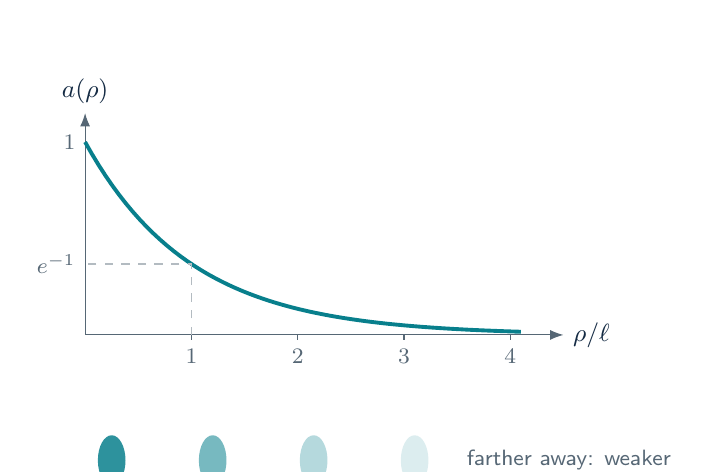
\begin{tikzpicture}[x=1.35cm,y=2.45cm]
  \draw[->,muted] (0,0)--(4.5,0) node[symbol,right] {$\rho/\ell$};
  \draw[->,muted] (0,0)--(0,1.15) node[symbol,above] {$a(\rho)$};
  \draw[teal,line width=1.4pt,domain=0:4.1,samples=65] plot (\x,{exp(-\x)});
  \draw[muted!45,dashed] (1,0)--(1,{exp(-1)})--(0,{exp(-1)});
  \node[note,left] at (0,1) {$1$};
  \node[note,left] at (0,{exp(-1)}) {$e^{-1}$};
  \foreach \x in {1,2,3,4}{\draw[muted] (\x,0)--(\x,-.025);\node[note,below] at (\x,-.025) {$\x$};}
  \foreach \x/\c in {0.25/teal!85,1.2/teal!55,2.15/teal!30,3.1/teal!14}{
    \fill[\c] (\x,-.65) circle (.13);
  }
  \node[note,anchor=west] at (3.5,-.65) {farther away: weaker};
\end{tikzpicture}
\captionof{figure}{Exponential attenuation with depth.
The points illustrate only relative brightness.}
\end{center}

\subsection{An Image from the Entire Volume}
For a simple transparent, additively luminous volume, define
\begin{modelbox}
\begin{equation}\label{eq:integral}
 I(\vct n;\tau)=\int_0^{\rho_{\max}}
 W(\rho;\tau)\,a(\rho)\,
 \F\!\left(z_\ast+\frac{\sigma(\vct n)}{Z(\rho)}\right)\dd\rho.
\end{equation}
\end{modelbox}
Integration is performed along a ray, not over the area of an entire spherical shell.
Therefore no area factor $4\pi\rho^2$ appears here. The weighting $W$ determines how
strongly a given depth contributes to the image. $W=1$ sums all shells; a normalized
narrow window around $\rho_c(\tau)$ preferentially shows one zoom level. If the
texture is continuous there, then in the limit of an increasingly narrow window,
$I\to a(\rho_c)T_{\rho_c}(\vct n)$.

\subsection{Numerical Representation and Brightness Bound}
A discrete representation with shell spacings $\Delta\rho_j$ is
\begin{equation}
 I(\vct n;\tau)\approx\sum_j
 W(\rho_j;\tau)a(\rho_j)T_{\rho_j}(\vct n)\,\Delta\rho_j.
\end{equation}
The factors $\Delta\rho_j$ prevent the image from becoming brighter merely because
more shells are sampled. For $W=1$ and every color component $k$,
\[
 0\le I_k\le\int_0^{\rho_{\max}}e^{-\rho/\ell}\dd\rho
 =\ell(1-e^{-\rho_{\max}/\ell})\le\ell.
\]
A fixed exposure and color mapping are then applied for display. A narrow depth
weighting also prevents many zoom levels from blending simultaneously into a
low-contrast average.

\newpage
\section{What Does It Mean That Every Point Is an Observation Center?}
\subsection{The Same Construction Rule Around Every Center}
For every $\vct o\in\R^3$, formula~\eqref{eq:field} defines an admissible model.
If the target point, orientation, and zoom law remain the same, then for every
translation $\vct b$,
\begin{equation}\label{eq:covariance}
 C_{\vct o+\vct b}(\vct x+\vct b)=C_{\vct o}(\vct x).
\end{equation}
That is: \emph{the family of models is translation-covariant.}
Every point can be the center of a shell volume constructed by the same rule.
Under such recentering, the field changes in the fixed world coordinate system.

\begin{center}
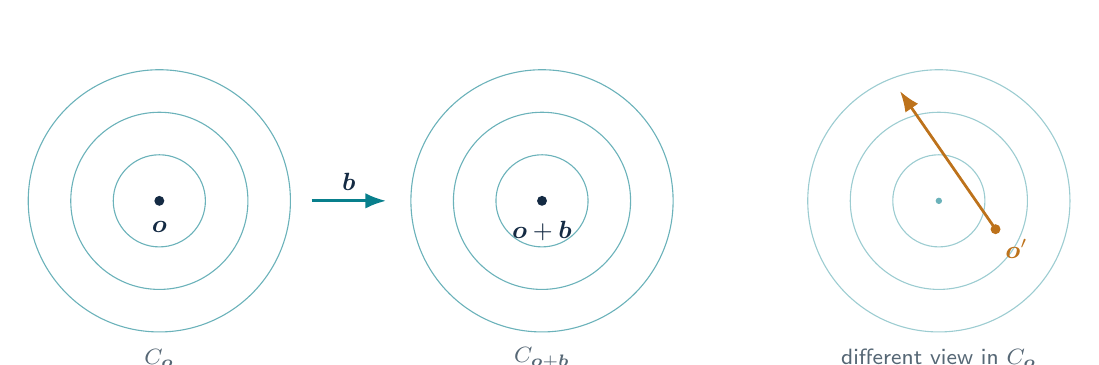
\begin{tikzpicture}[scale=.9]
  \begin{scope}[shift={(0,0)}]
    \foreach \r in {.65,1.25,1.85}\draw[teal!60] (0,0) circle (\r);
    \fill[navy] (0,0) circle (.07);
    \node[symbol,below] at (0,-.15) {$\vct o$};
    \node[note] at (0,-2.22) {$C_{\vct o}$};
  \end{scope}
  \draw[ray] (2.15,0)--(3.2,0) node[symbol,midway,above] {$\vct b$};
  \begin{scope}[shift={(5.4,0)}]
    \foreach \r in {.65,1.25,1.85}\draw[teal!60] (0,0) circle (\r);
    \fill[navy] (0,0) circle (.07);
    \node[symbol,below] at (0,-.15) {$\vct o+\vct b$};
    \node[note] at (0,-2.22) {$C_{\vct o+\vct b}$};
  \end{scope}
  \begin{scope}[shift={(11,0)}]
    \foreach \r in {.65,1.25,1.85}\draw[teal!40] (0,0) circle (\r);
    \fill[teal!60] (0,0) circle (.045);
    \fill[amber] (.8,-.4) circle (.07);
    \draw[->,amber,line width=1pt] (.8,-.4)--(-.55,1.55);
    \node[symbol,text=amber,below right] at (.8,-.4) {$\vct o'$};
    \node[note] at (0,-2.22) {different view in $C_{\vct o}$};
  \end{scope}
\end{tikzpicture}
\captionof{figure}{Left and center: the entire model is translated.
Right: another observer looks into the original, fixed volume.}
\end{center}

\subsection{Another Observer in a Fixed Volume}
If the world field $C_{\vct o}$ remains fixed and the observer is at $\vct o'$,
then the ray $\vct x(u)=\vct o'+u\vct n'$ passes through different shell intersections:
\begin{equation}
 \rho(u)=\|\vct o'-\vct o+u\vct n'\|,\qquad
 \vct n(u)=\frac{\vct o'-\vct o+u\vct n'}{\rho(u)}.
\end{equation}
In general, $\rho(u)\ne u$, and $\vct n(u)$ is not constant.
The new observer therefore does not see an identical concentric zoom sequence.

\subsection{Exact Equality and Statistical Homogeneity}
A fixed field satisfying $C(\vct x+\vct b)=C(\vct x)$ for \emph{all} translations
$\vct b$ would have to be constant: with $\vct b=\vct y-\vct x$, one immediately gets
$C(\vct y)=C(\vct x)$. A nonconstant shell fractal cannot satisfy this strong pointwise
condition. Statistical homogeneity, by contrast, means a translation-invariant
probability law; it would be an additional model requirement and does not guarantee
identical images.

\begin{modelbox}
The proposed model is a \textbf{three-dimensional field of continuously zoomed
spherical shells}. The center remains fixed when rotating and when selecting other
depths. The same construction rule can be applied around any center; this describes
a family of volumes.
\end{modelbox}

{\footnotesize\color{muted}
\textbf{Sources and model status.}
The Pratt definitions and the shell idea come from the conversation;
the iteration corresponds to the supplied renderer \texttt{render.cpp}.
The zoom law, attenuation, and image integration are explicit model choices here.\par
[1] NIST, \emph{DLMF}, Section 25.2: \url{https://dlmf.nist.gov/25.2}.\par
[2] J. C. Baez, \emph{The Octonions}, Section 3.3, Möbius transformations
of the Riemann sphere:
\url{https://math.ucr.edu/home/baez/octonions/node11.html}.
}
\end{document}
